\documentclass{article}
\usepackage{graphicx}
\usepackage{amsthm}
\usepackage{multicol}
\usepackage{vmargin}
\usepackage{authblk}
\usepackage{tocloft}



%-----set margins------------------

\setmargins{2.5cm}
{1.5cm}                       % margen superior
{16.5cm}                      % anchura del texto
{23.40cm}                     % altura del texto
{10pt}                        % altura de los encabezados
{1cm}                         % espacio entre el texto y los encabezados
{0pt}                         % altura del pie de página
{2cm}            


\begin{document}

\title{Site percolation and critical probability}

\author[1]{
  David F. Bambagüe
}
\affil[1]{
    dbambague@unal.edu.co
}
\author[2]{
  Joel B. Ortiz
}
\affil[2]{
    jobernalo@unal.edu.co
}
\author[3]{
  Juan D. Bernal
}
\affil[3]{
    jbeltranp@una.edu.co
}
\author[4]{
  Danny J. Perilla
}
\affil[4]{
    djperillam@unal.edu.co
}

\affil[1-4]{Departamento de Física, Universidad Nacional de Colombia, Bogotá, Colombia}
\date{\today}

\maketitle

\begin{abstract}
 En el presente estudio se pretende estudiar la percolación de sitio a través de una réplica computacional. Se encuentra que variando los parámetros de la simulación la probabilidad crítica es $p_c=0.59$, valor que se aproxima mejor entre mayor es el tamaño del sistema. Además, se encuentra que el tamaño promedio del cluster percolante más grande normalizado al tamaño del sistema presenta un punto de inflexión en la $p_c$ y luego de un valor de $p=0.7$ todos los valores de tamaño promedio son los mismos, sin importar el tamaño de la matriz, el cual además crece linealmente a partir de este valor. Finalmente, el profiling del código evidencia que el programa ejecutado escala cúbicamente. 
 
\noindent\textit{Palabras clave}: percolación de sitio, probabilidad crítica, simulación, profiling, cluster percolante, optimización.
\end{abstract}
\vspace{-1cm}
\begin{figure}[h]
    \begin{center}
    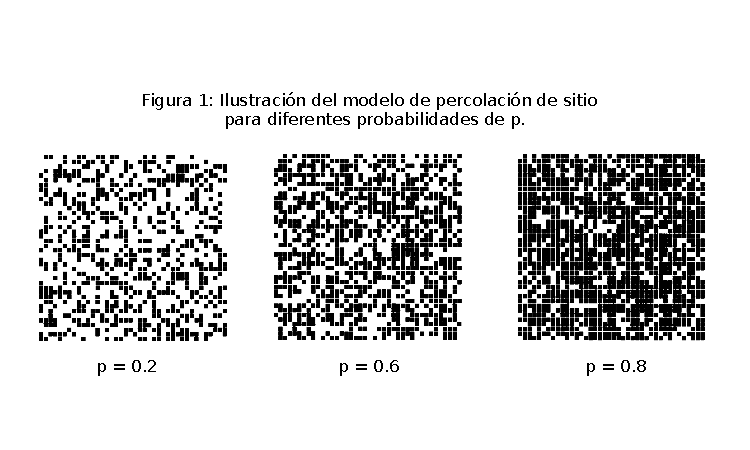
\includegraphics[scale=1]{percolation.pdf}
    \label{fig1}
    \end{center}
\end{figure}
%\caption{Ilustración del Modelo de percolación de sitio para diferentes probabilidades de llenado $p$ }
\vspace{-1cm}
\begin{multicols}{2}

\section{Introducción}


La percolación es un fenómeno relacionado con el paso de una sustancia a través de una frontera, o dicho de una forma más general, se trata de la transmisión de una propiedad a través de un medio, donde se tienen en cuenta las propiedades del medio. Este fenómeno lo podemos ver en diferentes situaciones, como por ejemplo el agua pasando a través de granos de café en una cafetera, o la extracción de petróleo del suelo, haciéndolo percolar a través del medio poroso bajo el que se encuentra.  Por lo que es un fenómeno de gran interés para el estudio físico, y que ha tomado gran relevancia en la actualidad (Giordano, 1997).  


Históricamente, la teoría de la percolación se remonta a Flory y Stock Mayer, quienes durante la segunda guerra mundial describieron como las moléculas ramificadas forman macromoléculas cada vez más grandes, formando así una red de enlaces químicos que abarca todo el sistema (Sahini, 2003). No obstante, el término percolación fue acuñado en una publicación de Broadbent y Hammersley (Broadbent, 1954) quienes hicieron un trabajo con un enfoque más matemático donde se le dio la importancia a las propiedades aleatorias de un fluido defiriendo de la teoría convencional de difusión. Más adelante, la incursión de los métodos computacionales ayudaron al desarrollo de modelos más complejos a través de soluciones numéricas. Uno de los algoritmos más rápidos en la actualidad uno de los algoritmos fue publicado en 2000 por Mark Newman y Robert Ziff (Newman, 2000). La percolación está además íntimamente relacionada con los  fractales, transiciones de fase e invariancia de escala. 


\subsection{Percolación de sitio}

La percolación de sitio es un modelo donde se considera una red de puntos regulares que forman una malla en un espacio euclídeo bidimensional. Como lo que se quiere estudiar es cuando pasa o no la sustancia a través de la frontera que en este caso estaría representada por la malla de puntos, se declara o define una probabilidad $p$ de llenado a cada punto y $1-p$ de que no lo esté. Luego se examina cada celda de la matriz, donde se determina si sus vecinos inmediatos (arriba, abajo, y los lados) están o no llenos y por ende conectados entre sí, es decir,  que ambos puntos permitan el paso del fluido. Luego, si vemos todos los puntos de la red podremos estudiar si se forman caminos entre los diferentes puntos, dichos caminos son denominados clusters que serán o no extensos dependiendo de la probabilidad $p$ de llenado que se asigne al sistema, así, si la probabilidad es pequeña no se podrán hacer clusters demasiado grandes (o ninguno si $p$ es demasiado pequeña), por lo que si $p$ es lo suficientemente grande existirá el caso que el cluster atraviese todo el sistema, lo que se denomina un cluster percolante. 

En el presente trabajo se pretende estudiar este modelo de percolación el cual es el más simple. Esto se desarrollará a través del estudio de un modelo computacional sencillo, variando los diferentes parámetros como el tamaño de malla y la probabilidad de llenado $p$, con el fin de determinar el valor de la probabilidad crítica $p_c$: esta se define como el valor mínimo desde la cual (muy probablemente) siempre aparece un cluster percolante. El valor de la $p_c$ para el modelo expuesto no tiene una solución analítica, por lo que se requieren simulaciones repetidas para estimarlo.     También se estudia cuál es el promedio del cluster percolante más grande dados $p$ y $L$ donde $L\times L$ es el tamaño de la matriz. Finalmente, se pretende examinar qué tan eficiente es el código en cuestión y qué alcance tiene la resolución planteada en el código expuesto.

\section{Desarrollo del código} 

El problema central en la realización de código radicó en el conteo de manera precisa de los clusters para luego clasificarlos como percolantes o no. Inicialmente, se propuso una lectura  continua de la matriz, esto se hizo por medio de bastantes if y for anidados dentro de las funciones propuestas inicialmente en el código, la matriz que representaba la malla del sistema estaba declarada en la representación de un vector de vectores. No obstante, además de ser ineficiente el uso de este tipo te matrices y de conteo por medio de condiciones complejas y poco prácticas, se presentaban problemas en el conteo del número total de elementos pertenecientes a la percolación, pues no se reconocía la extensión completa de aquellos que poseían bifurcaciones, esto se evidenció durante la impresión de distintas matrices de tamaños relativamente pequeños ($L<10$) que permitieran un conteo manual del tamaño de una percolación.  Únicamente se verificaba la existencia de percolaciones verticales en la matriz original por lo que para las horizontales se optó por tomar la transpuesta.

Por esta razón se optó por un método recursivo el cual sí era robusto frente a los clusters ramificados. Dicho algoritmo recibía unas coordenadas, le asignaba valor cero a esa casilla de la matriz (para evitar el sobreconteo) y verificaba todos sus vecinos para actualizar el conteo del tamaño y volver a llamar la función en aquellos vecinos con valor de celda igual a 1, esta forma de código reducía la complejidad del código y hacía de una representación unidimensional de la matriz para tener los datos contiguos en memoria, así como también se propició el uso de una matriz extendida, es decir, una matriz rodeada de ceros para evitar el acceso a elementos no inicializados. Sin embargo, eliminar las casillas ya visitadas generaba conflictos al revisar los percolantes horizontales, ya que si estuviésemos haciendo el conteo de un cluster vertical que fuera una rama de un percolante horizontal (forma de T) el conteo vertical anularía o borraría el percolante horizontal. Esto se solucionó haciendo una copia de la matriz antes de analizarla y corriendo posteriormente el algoritmo sobre su transpuesta.

No obstante, el análisis de matrices $n\times n$ de más $n=400$ con probabilidades de llenado mayores a $p=0.6$ causaba segmentación fault. Un primer análisis con sanitaizers y valgrind era insuficiente para encontrar el problema; sin embargo, a través de la indagación independiente, se encontró que la  recursividad era el origen del problema, ya que saturaba el stack de memoria disponible dada la gran cantidad de autollamados para el análisis de los clusters de la matriz. Se intentó aumentar el tamaño del stack usando ulimit en la terminal, pero aún con su tamaño máximo, el problema del segmentation fault no se solucionó.  

Finalmente, se descartó el uso de recursividad usando estructuras que guardaban las coordenadas de los vecinos con valor de celda igual a 1 mientras que se borraban de sí misma las coordenadas ya visitadas, además un bucle while se ejecutaba hasta que la estructura estuviese vacía por lo que se recorrían todos los elementos de cada cluster sin reconteo y sin problemas con las bifurcaciones. Este modelo con estructuras y un bucle resolvió el segmentation fault, pudiendo emular sistemas de más de $n=1000$.

Otra optimización que se realizó durante el proceso fue la utilización de librería eigen, una librería que es especializada en la representación y manipulación de matrices. El llenado de la matriz, su inspección y algunas operaciones, eran mucho más eficientes, así como también el cálculo de la matriz transpuesta para los conteos horizontales y el empleo de doble índice que es más fácil de leer.  Al final el código que inicialmente tenía una gran cantidad de líneas y funciones (7) se redujo a uno con simplemente 2 funciones para la simulación.	  

\section{Profiling}

Un análisis más concreto sobre el código se realizó por medio del profiling. Para este se tuvo en cuenta la bandera de optimización, $01$ la cual ,como se evidencia en la gráfica, mejora el rendimiento en casi un $22\%$ con respecto a no usarla.

Por otro lado, el profiling revela la cantidad de tiempo que gasta cada función en el código. Como se evidencia en la gráfica 2 la función perco-size gasta la mayor parte del tiempo (un $72\%$) de ejecución del código. Esta función se encarga realizar el conteo de los elementos de los clusters y clasificarlos como percolante o no, por lo que tiene sentido que sea la de mayor tiempo de cómputo, dado que fue el eje central del código.

Le sigue con un $17\%$ del tiempo de cómputo la función emplace-back sobre la estructura Vecinos que era la encargada de guardar las coordenadas de las casillas adyacentes con valor de celda igual a 1. A su vez, esta función de la estructura tiene el $80\%$ de las llamadas. Su explicación es que la cantidad de llamadas para llenar la estructura será mayor o igual a la suma de los tamaños de todos los clusters que comiencen desde la parte superior de la matriz y menor o igual a la suma de los tamaños de todos los clusters que comiencen desde la parte superior o izquierda de la matriz. Finalmente, con un $6\%$ y $4\%$ del tiempo lo tienen las funciones mersenne-twister y la función push-back. La primera es una herramienta que utiliza un algoritmo encargado de producir números aleatorios, que se utiliza para la asignación de los valores de cada entrada de la matriz con base en una distribución Bernoulli $B(p)$. La función tiene tantas llamadas como la cantidad de elementos de la matriz, por lo que posee el $20\%$ de las llamadas en el programa. Y la segunda se encarga del llenado de la estructura, por lo que tiene el $1.21\%$ de las llamadas. La segunda y la cuarta función tienen funciones complementarias en el manejo de la estructura utilizada.

El resto del código hace prácticamente un gasto casi nulo del tiempo de ejecución del código en comparación con las funciones antes mencionadas.


\end{multicols}{}

\begin{figure}[h!]
    \begin{center}
    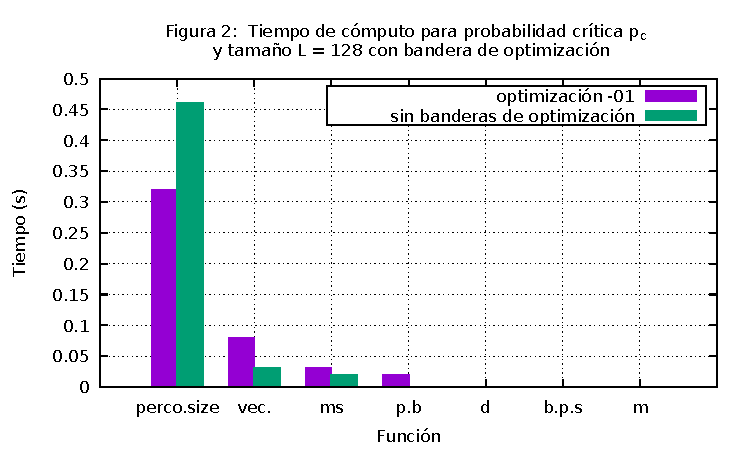
\includegraphics[scale=1]{profile0.pdf}
    \end{center}
\end{figure}

\begin{figure}[h!]
\begin{center}
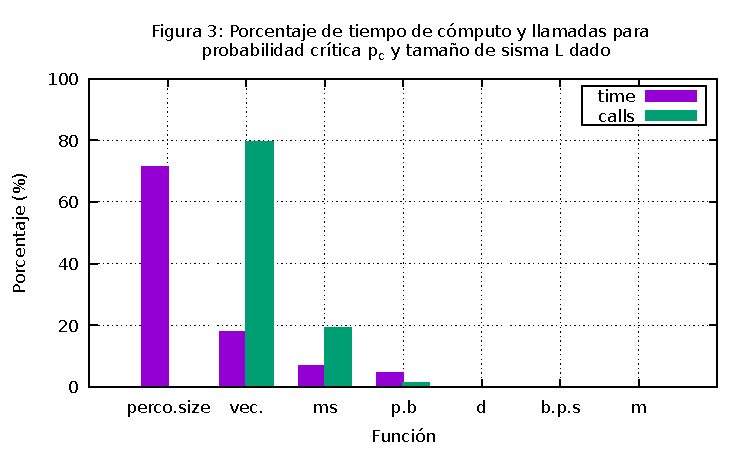
\includegraphics[scale=1]{profile1.pdf}
\label{fig2}
\end{center}
\end{figure}

\begin{multicols}{2}

\section{Resultados} 


En la figura 4 se muestra la probabilidad $P$  de encontrar un cluster percolante en función de la probabilidad de llenado $p$. Se varió el tamaño del sistema $L$ para 5 valores: 32, 64, 128, 256 y 512. Observe que conforme crece el tamaño del sistema, el rango de valores en el cual eventualmente ocurre un cluster percolante a los alrededores de la probabilidad crítica se hace más estrecho y se va asemejando a una función escalón unitario con discontinuidad de salto en la probabilidad crítica, que se da en el valor aproximado dé $0.59$. Por lo que entre más grande es el tamaño $L$ es más certero encontrar dicha probabilidad crítica. Además, note que para probabilidades de llenado mayores a $p=0.65$ la probabilidad de que exista un cluster percolante es casi $1$ sin importar el tamaño del sistema.

Por otro lado, la figura 4 representa el promedio (normalizado al tamaño de la matriz $L \times L$) del tamaño del cluster percolante más grande en función de la probabilidad de llenado $p$. En esta figura también se ve la acción de la probabilidad crítica, $p_c$ vemos que previo a este valor  los tamaños promedios decrecen a mayor es el valor de $L$, sin embargo pasado este valor crítico la relación se invierte. Gráficamente, se puede ver que en este valor de probabilidad crítico aparece un punto de inflexión, el cual es más evidente a mayor es el tamaño del sistema. Asimismo, luego de una probabilidad de $p=0.7$ los tamaños promedios convergen mostrando valores muy similares que crecen aparentemente de forma lineal. 

El escalamiento del tiempo en función del tamaño del sistema se presenta en la figura 6 donde se hace por medio de una representación log-log donde se evidencia que la relación tamaño-tiempo es una línea recta, por lo que el crecimiento del tiempo es potencial, así al hacer un ajuste potencial de los datos se encuentran las ecuaciones (1) y (2) que corresponden a las relaciones de la compilación con $O1$ y $O3$ respectivamente. Vemos además que a pesar de utilizar las banderas de optimización $01$ y $03$ no se percibe cambio alguno entre estas, por lo que muy probablemente las optimizaciones adicionales aplicadas en $03$ no son significantes y por ende sin mayor utilidad.


\begin{equation}
        F(x) = (1.9 \pm 0.3)\times10^{-7}x^{3.20\pm0.02}
\end{equation}

\begin{equation}
        G(x) =(1.87 \pm 0.5)\times10^{-7}x^{3.21\pm0.04}
\end{equation}


\end{multicols}{}


\begin{figure}[h!]
    \begin{center}
    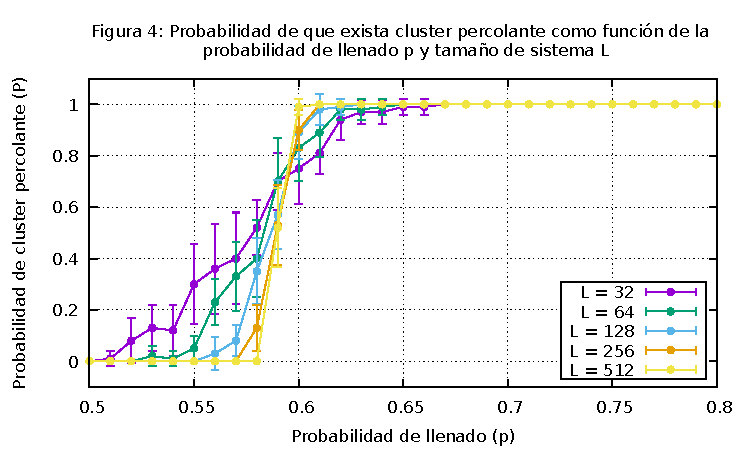
\includegraphics[scale=0.9]{prob.pdf}
    \end{center}
\end{figure}

\begin{figure}[h!]
    \begin{center}
    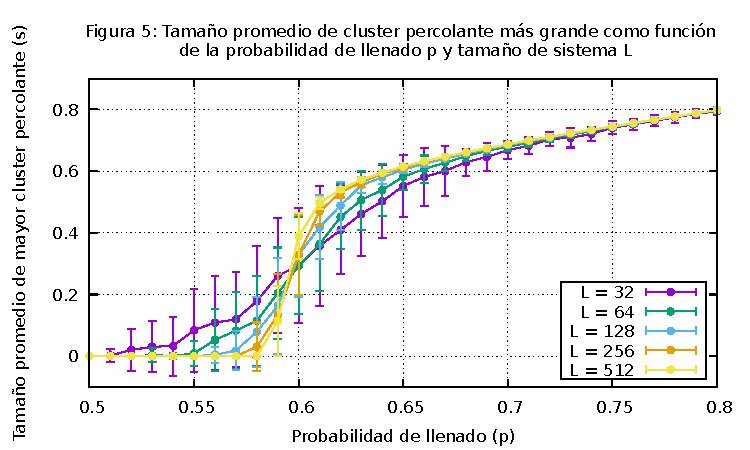
\includegraphics[scale=0.9]{size.pdf}
    \end{center}
\end{figure}

\begin{figure}[h!]
    \begin{center}
    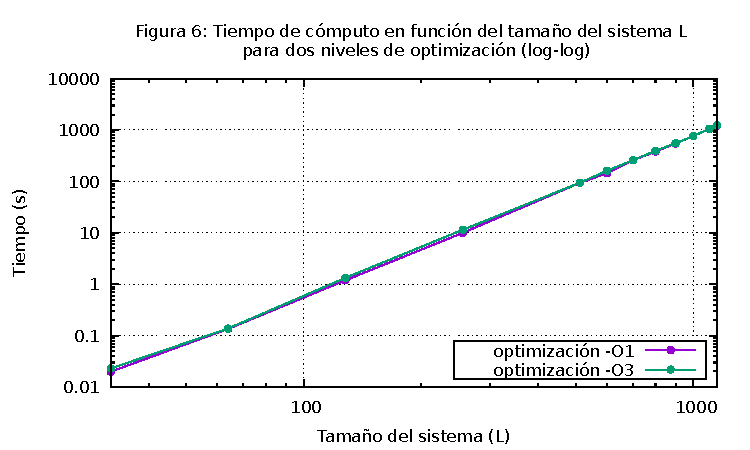
\includegraphics[scale=0.9]{time.pdf}
    \end{center}
\end{figure}

\begin{multicols}{2}
\section{Conclusiones}

La probabilidad crítica converge a un valor de $p_c=0.59$ a medida que tamaño del sistema aumenta, pues la muestra es mayor y la medición probabilística es más certera. También para este valor de probabilidad crítica aparece un punto de inflexión en la gráfica del tamaño promedio del cluster percolante. Los valores en esta gráfica convergen para cualquier valor de malla luego de una $p=0.7$ y se comporta de forma lineal.

El código realizado es bastante óptimo, solo mejora en un $18\%$ el rendimiento para la bandera de optimización $01$ y para las demás no mejora significativamente. Por otro lado, el tiempo de cómputo escala de forma potencial, con un exponente de $3.20\pm0.02$.



\section{Referencias}

\noindent [1] Giordano, N.; Nakanishi, H. (1997). Computational Physics (2.a ed., Vol. 1,pp 195-198). Prentice Hall.\\

\noindent [2] Sahini, M.; Sahimi, M. (2003-07-13). Aplicaciones de la teoría de la percolación. Prensa CRC.\\
  
\noindent [3] Broadbent, S. y Hammersley, J. (1957). Procesos de percolación: I. Cristales y laberintos. Procedimientos matemáticos de la Sociedad Filosófica de Cambridge, 53 (3), 629-641 .\\
  
\noindent [4] Newman, Marc Ziff, Robert (2000). ¨Efficient Monte Carlo Algorithm and High-Precision Results for Percolation". Physical Review Letters.
  

  
  
\end{multicols}{}

\end{document}
